\section {Formularea problemei}

In urma studiului de piata din capitolul anterior am concluzionat ca exista un segment de utilizatori care ar fi interesati in a folosi un astfel de sistem. In cele ce urmeaza voi prezenta 

\section {Studiu asupra realizărilor similare din domeniu}


\subsection {Videx UK}

Interfoanele \acrshort{gsm} de la Videx sunt conectate la reteaua mobila de telefonie si permit operarea unei porti prin intermediul unui releu. Ele necesita doar o sursa de curent externa, o antena si o cartela \acrfull{sim} pentru a opera.

\begin{figure}[h!]
  \centering
  \fbox {
    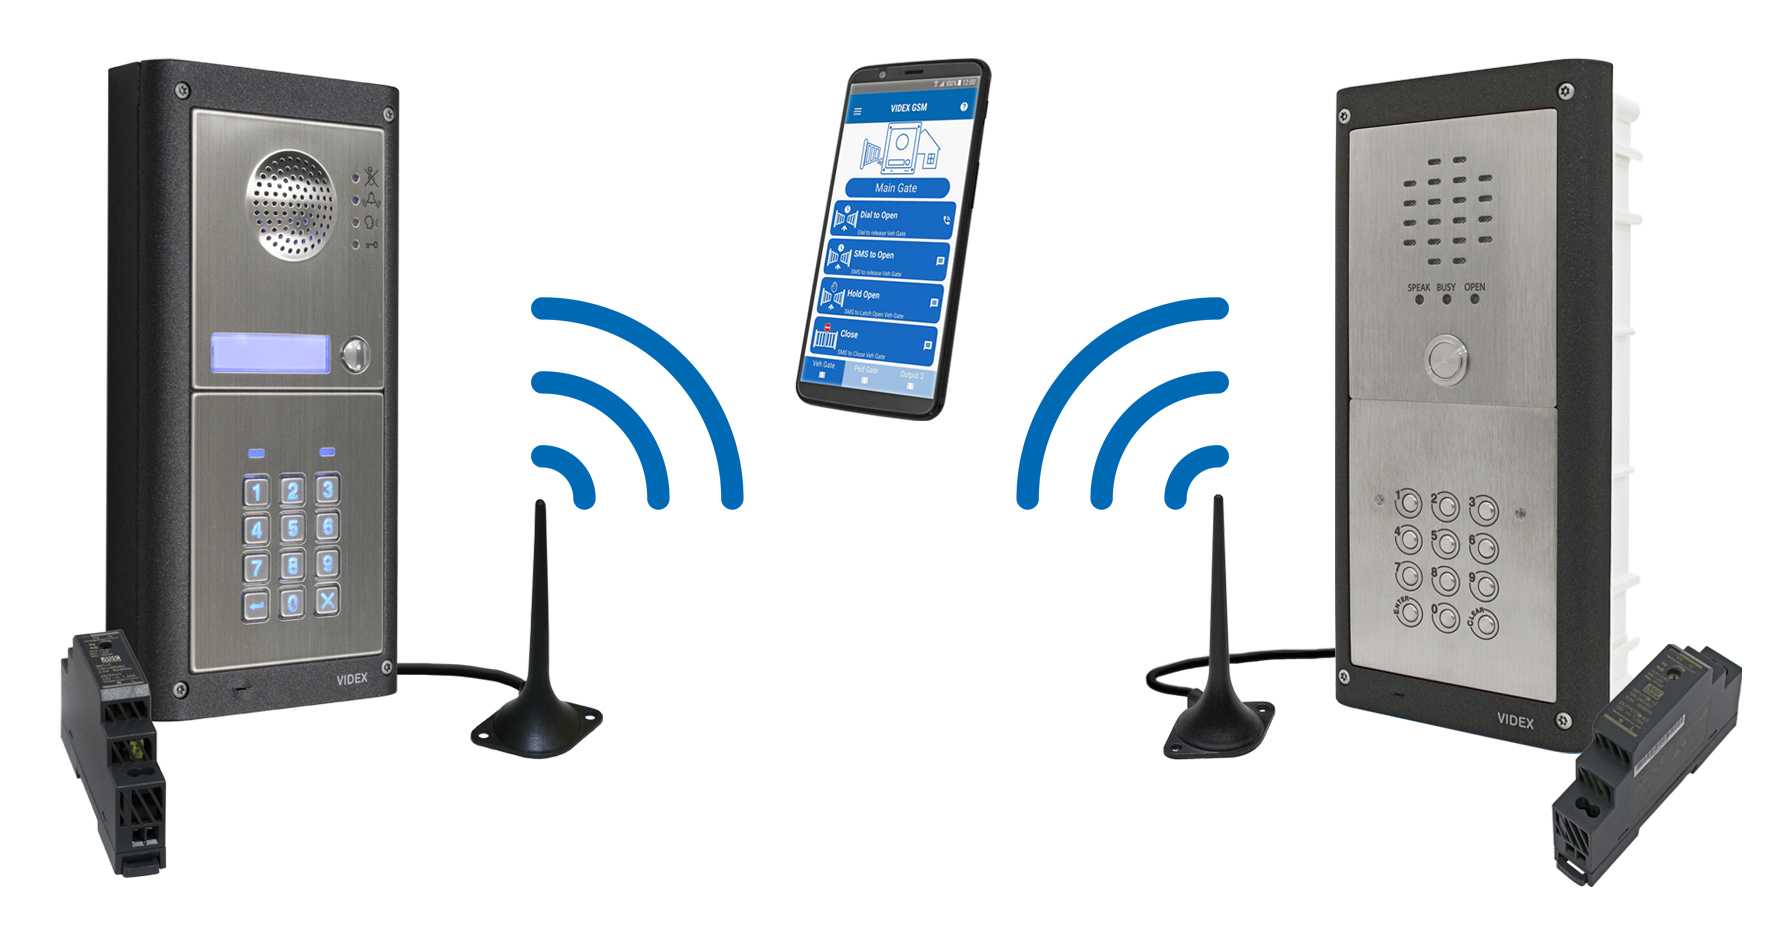
\includegraphics[width=0.6\textwidth]{02/01_gsm_system.jpg}  
  }
  \caption{Sistem interfon Videx GSM \cite{VidexUk}}
\end{figure}

Printre functionalitatile principale se numara:
\begin{itemize}
  \item Poate include un cititor de carduri \acrshort{rfid} si cheie
  \item Versiune rezistenta la vandalism
  \item Pana la 4 numere de telefon per apartament, pentru redundanta. In cazul in care primul numar nu se poate apela sau nu raspunde, se va incerca urmatorul numar programat
  \item Ofera aplicatie Android si iOS pentru programat unitatea
\end{itemize}

Dezavantaje:

\begin{itemize}
  \item Nu ofera integrare cu servicii din reteaua \acrshort{iot}
\end{itemize}

\subsection {Google Nest x Yale Lock}

\begin{figure}[h!]
  \centering
  \fbox {
    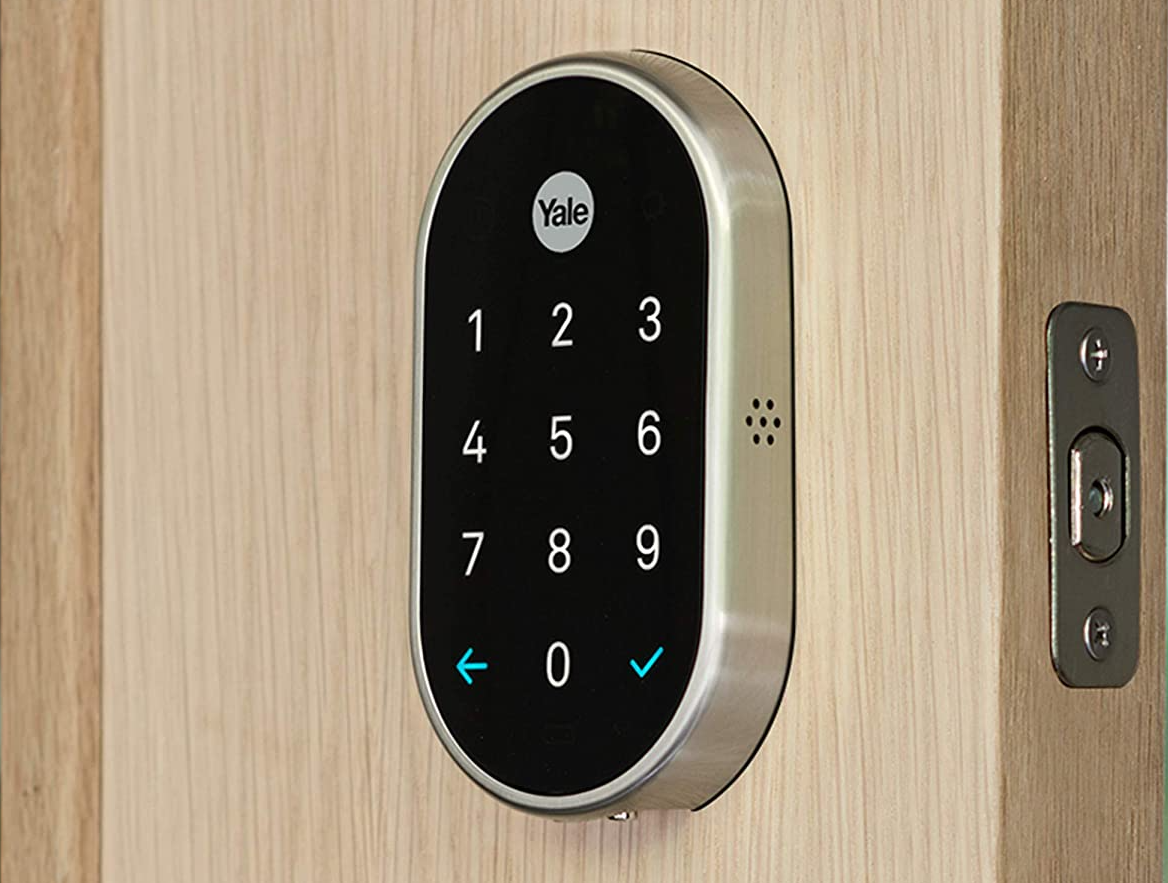
\includegraphics[width=0.6\textwidth]{02/02_iot_system.png}  
  }
  \caption{Next x Yale Lock \cite{YaleLock}}
\end{figure}

Avantaje:
\begin{itemize}
  \item Permite accesul prin intermediul unui PIN ales de utilizator
  \item Ofera alerte cand cineva inchide sau deschide usa
  \item Ofera integrare cu Google Home si Nest Home
\end{itemize}

Dezavantaje:
\begin{itemize}
  \item Are nevoie de 4 baterii tip AA pentru a functiona
  \item Nu are acces cu cheie sau cartela
  \item Nu are versiune rezistenta
\end{itemize}


\subsection {Level Lock - Touch Edition}

Level Lock este o incuietoare inteligenta de tip zavor. Are un design minimalist si ascunde partea electronica in interiorul usii pentru mai multa securitate.

\begin{figure}[h!]
  \centering
  \fbox {
    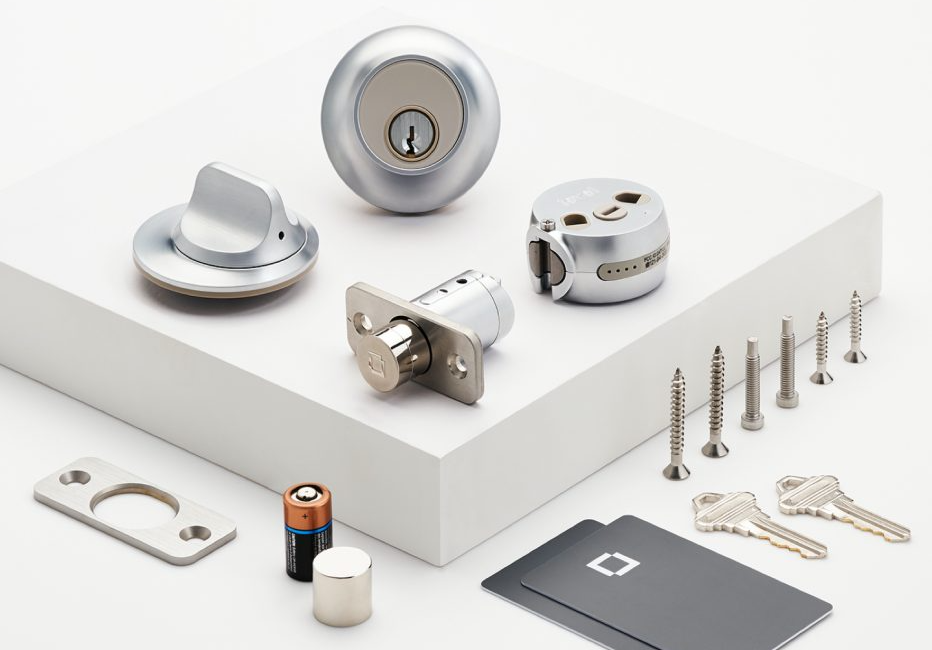
\includegraphics[width=0.6\textwidth]{02/03_iot_system.jpg}  
  }
  \caption{Level Lock \cite{LevelLock}}
\end{figure}

Avantaje:
\begin{itemize}
  \item Multiple modalitati de acces, printre care: amprenta, PIN, 
  \item Ofera alerte cand cineva inchide sau deschide usa
  \item Ofera integrare cu Google Home si Nest Home
\end{itemize}


\href{https://www.apple.com/shop/product/HPFY2ZM/A/level-lock-touch-edition?fnode=648f1e74ceef61358f897cd3f7cdb053262fd38bbffcd78c49f653a17d8b06312e1d22bd76ab325e817a33264364be774af0cc44d3ce62d8efcc0301ce4fbedabf176781e07520161f01ce6f69b6cb8ad4774b3cc302ff5d1dfc2d1524cf313aaeb1b1323955c95e3319224270e9b632&fs=fh%3D482b%252B45ae}{Apple listing}

\subsection {Comparatii}

Produsele de mai sus adreseaza probleme diferite, dar incearca sa ofere functionalitati similare. Sistemul oferit de Videx Security prezinta un design rezistent, dar familiar tuturor utilizatorilor si este destinat cladirilor cu mai multi locatari. In contrast, cele doua incuietori inteligente ofera o integrare avansata in reteaua \acrshort{iot} si multiple cai de acces, dar sunt destinate unei singure locuinte.

Incuietoarea de la Yale prezinta cea mai inovativa abordare a acestul design prin decizia deliberata de a nu oferi posibilitatea de acces cu cheie. Astfel, simplifica partea mecanica eliminand singura cale de acces din exterior catre mecanismul incuitorii.

Produsul celor de la Videx Security se bazeaza pe o tehnologie utilizata la scara larga si prin urmare prezinta 

Din lipsa unor standarde in domeniu, dispozitivele noi sufera de alte tipuri de probleme:
\cite{Bitdefender2016IoT}

\section {Stabilirea cerințelor funcționale si nefuncționale ale sistemului}

\subsection{Controlul accesului intr-o cladire}

Scopul principal al acestui sistem este de a oferi sau nu acces intr-o incinta, prin urmare consider aceasta cea mai importanta cerinta functionala.

\subsection{Expunerea unui serviciu REST pentru interfatarea cu alte sisteme}

Expunerea si abstractizarea terminalului \acrshort{pots} este realizata printr-un set de servicii \acrfull{rest} care controleaza starea sa. Acest lucru ne permite interfatarea cu aplicatia mobila, interfata de administrare web si alte servicii precum Google Home/Google Assistant/Apple HomeKit.

\subsection{Implementarea unei functii pentru raspuns automat}

Aceasta functie va permite utilizatorului sa stabileasca o perioada de timp pentru care sistemul va oferi accesul neconditionat.

\subsection{Dezvoltarea unui client mobil Android}

Principalul client care va interactiona cu serviciile \acrshort{rest} va fi aplicatia mobila ce va avea rolul de a notifica userul cand ii suna interfonul si de a controla starea sistemului.

\subsection{Control granular asupra datelor stocate}

Arhitectura aplicatiei necesita interactiunea cu o baza de date, care poate fi tinuta in cloud, pentru convenabilitate sau local.
Folosind tehnologii de containerizare precum Docker, putem stoca baza de date local, informatiile fiind stocate intr-un mediu controlat.

\subsection{Criptarea comunicatiilor cu serviciile web}

Avand in vedere nivelul de acces pe care l-ar oferi un exploit al acestei solutii, comunicatiile intre server si clienti trebuie realizate printr-un canal criptat de tip \acrfull{ssl}. Credentialele userului si ulterior tokenul de acces trebuie trimise doar dupa verificarea autenticitatii serverului si a pachetelor trimise.

\subsection{Oferirea si revocarea accesului la sistem}

Dorim de exemplu sa oferim acces neconditionat unui prieten apropiat pentru a intra in bloc fara a mai suna la interfon. De asemenea ar trebui sa putem realiza si inversul acestei operatii.

\subsection{Expunerea unui flux duplex audio prin tehnologia VoIP}

Pasul final in dezvoltarea acestui sistem ar fi interfatarea cu un \acrfull{adc} si un \acrfull{dac} si expunerea streamurilor de date prin \acrfull{voip}
